\documentclass[../Main.tex]{subfiles} 
\begin{document}

\section{Geo location attempt }
As stated in the previous chapter, the foundation of all calculations in the regional word attempt is a list of a few hundred words that appear more likely in a specific region. 
Although this list and their probability distribution is based on scientific research it markes the weak spot of this attempt for number of reasons. For example people in a specific region use a typically word in their everyday language while speaking to their friends or family, but there is no proof that this people also use this words in their written language, even if it is only their private Twitter account. In addition, the list is way to short to cover only fraction of the words, people use on Twitter, so the end results mostly rely on the data that is generated in main loop of the algorithm.

We seem to have no other choice but to trust this generated values, so we had the idea of skipping the manually created word list and use an automatically created based on a corpus of Tweets with a geo location instead. \\
Before entering the main loop, we had to write another algorithm that learns the distribution on all seven regions for all the words in the corpus. This way we are generating a list of words that covers nearly all the words.
\begin{figure}
  \begin{center}
   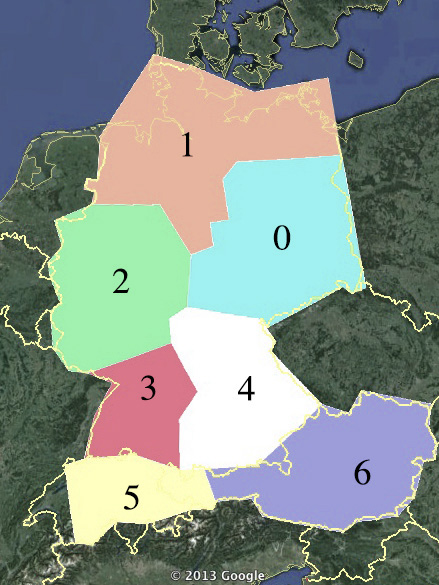
\includegraphics[width=0.5\columnwidth]{../img/polygone_satt.jpg}
    \caption{\label{geo_polymap} Map of the regions and their index represented as polygons}
  \end{center}
\end{figure}
In order to classify a tweet, that has a geo location, we had struggled to find a good way to represent the seven regions in a way, that we could easily check from which of them a Tweet was sent. After a few unsuccessful approaches, we decided to define polygons for the regions that are not overlapping each other, but also leave no gaps between them. For the value of the points we simply used their longitude and latitude coordinates, that can be represented as floats.  
We did not implement a point-in-polygon algorithm ourself, but used the version found here [SOURCE] instead. 
To find out from which region a tweet was sent, we iterate over all regions and return the first one, where the point-in-polygon function returns true.
In this first step, the Tweet-vector consists only of zeros and a one for the feature standing for the region it was sent from. 

Let's assume that the coordinates of some Tweet reveal, that its region is "Westdeutschland", represented by the index $3$.
Therefore the Tweet-vector is $(0,0,1,0,0,0,0)$. 
The next step consists of iterating over all token in the tweet and add the Tweet-vector to their word-vectors. To put it simply, we increase the counter for the specific feature of all occurring tokens by one. 
In the final step, we iterate over all word-vectors and use our \texttt{normalize()}-function to attain the probability distribution, how likely it is that the token is used in a specific region. Because of this normalization, the format of the outcome is comparable to the input list in the regional-word attempt and we can use the main part of the algorithm without having to adjust it.

\begin{figure}
\centering $\textrm{Example Tweet: } d = \textrm{'Hello Twitter!'} \textrm{ from the region 'Westdeutschland'.}$
 \begin{align*}
    \vec{t}_{hello} &= (1,3,2,5,2,1,0) \\
     \vec{t}_{twitter} &= (0,0,0,0,0,0,0) \\
      \vec{d} &= (0,0,1,0,0,0,0) \\
     \vec{t}_{hello}' &= \vec{t}_{hello} + \vec{d} =  (1,3,3,5,2,1,0) \\
    \vec{t}_{twitter} ' &= \vec{t}_{twitter} + \vec{d} = (0,0,1,0,0,0,0) \\
     \texttt{normalize(}\vec{t}'_{hello}\texttt{)} &= (0.04, 0.13, 0.13, 0.22, 0009, 0.04, 0) \\
     \texttt{normalize(}\vec{t}'_{twitter}\texttt{)} &= (0,0,1,0,0,0,0)
  \end{align*}
  \caption{Example for the creation of the initial word-vectors}
  \label{geo_example1}
\end{figure}

\subsection{Source of data}
The datasets used for the generation of the first word-vectors have been extracted from the Scheffler-corpus using the same classification function as in the main program. Although the corpus mostly consist of German Tweets (filtered with \emph{LangID}), about 20\% of the Tweets with geo-location have not been sent from one of the defined regions and therefore have been ignored. \\
We created balanced sets, where the amount of  Tweets are the same for all regions. Because the fewest number of Tweets (8787) came from region 6, 'Austria', we ended up with only 61509 Tweets for all regions. 

In order to create a gold-standard, we substracted 150 Tweets from each region, leaving us 60459 for the training. \\
Our assumption was, that datasets of different sizes lead to different results and we wondered, how it would effect the accuracy, if we would use the same data for the creation of the word-vectors and for the main-algorithm. Therefore we created three balanced sets, one unbalanced set of all geo annotated Tweets and as a reference one huge set of normal Tweets. Of course none of these sets contain any Tweets from the gold-standard-set.
 \begin{enumerate}
\item \emph{balanced-21k} with 3000 Tweets from each region.
\item \emph{balanced-39k} consisting of the remaining 39456 Tweets
\item \emph{balanced-61k} combining the both previous sets. 
\item \emph{geo-175k} with all Tweets from the corpus that were sent from one of the defined regions. Not balanced.
\item \emph{all-1500k} contains 1.5 million mostly not geo annotated Tweets.
\end{enumerate}
\subsection{Experiments}
\subsubsection{Dataset combinations}
\begin{table}[b]
    \begin{tabular}{|l|lllll|}
    \hline
    Geo dataset     & balanced-21k & balanced-39k & balanced-61k & geo-175k & all-1500k \\ \hline
    balanced-21k    & 0.319        & 0.308        & 0.304        & 0.307           & 0.308       \\
    balanced-39k    & 0.306        & 0.353       & \textbf{0.345}        & \textbf{0.368 }          & 0.306       \\
    balanced-61k    & \textbf{0.336}        & \textbf{0.361}        & 0.344        &0.360           & 0.332       \\
    unbalanced-175k & 0.303        & 0.343        & 0.322        & 0.352           & \textbf{0.340}       \\ \hline
    \end{tabular} \\

  Calculation method: \textit{Normalized}; Stopwords: \textit{Top 200}; Loops: \textit{1}; Estimated amount of non-regional Tweets: \textit{60\%}, leading to a similarity threshold between \textit{0.999} and \textit{0.991}, depending on the dataset.
  \caption{Comparrision of the combination of all datasets}
  \label{geo_datasets}
\end{table}

In order to give a solid foundation which data we should use in further experiments, we started to compare the combination of the five datasets we created. We wondered, how it would affect the accuracy, if we would for example train the geo-algorithm with a small set of geo-annotated data but use a very big set of Tweets for the learning of the word-vectors in the loop of the main-algorithm. Another question was, what results we would get, if the data in the main-algorithm contains Tweets, that have been used in the geo-algorithm before. 

Our expectation was in general, that the accuracy would rise, the more data we use and that the reuse of Tweets in the main-algorithm would lower it, because this data already had an effect and using it again would not change anything.

Unsurprisingly, using the smallest set, \emph{balanced-21k}, for the training of the geo-algorithm nearly always produced the lowest accuracy. \\
But our hypothesis about the reuse of data was falsified:  The combination of the \emph{balanced-39k} set for the learning in the geo-algorithm and \emph{balanced-61k} for the main-algorithm generated the third best result with an accuracy of 0.345.

Also we discovered, that the use of balanced data  in the geo-algorithm, where all regions are represented by the same amount of documents, is crucial for good results. Having a look at the row for the \emph{unbalanced-175k}, it produces a very bad accuracy. Even in combination with the set containing 1.5 million Tweets (\emph{all-1500k}), it marks the second last rank.

This experiment showed us, that we should use the \emph{balanced-39k}-set for the training of the geo-algorithm and the \emph{geo-175k}-set for the main-algorithm, because it generated the best accuracy of 0.365. We were surprised, that the combination \emph{balanced-39k} / \emph{all-1500k} had a worse result, but interpreted it as a result of the unfiltered data of the \emph{all-1500k}-set.

\subsubsection{Comparission of different stopword-lists}
\begin{figure}
\begin{center}
\begin{tikzpicture}
        \begin{axis}[
                              width=0.9\columnwidth,
                              height=0.3\textheight,
                              symbolic x coords={200 stopwords, 500 stopwords, 750 stopwords, 1000 stopwords},
                              xtick=data,
                              ylabel=accuracy,
                              bar width=40
          ]
            \addplot[ybar,  postaction={ pattern=north east lines  }] coordinates {
               (200 stopwords, 0.368)
	      (500 stopwords, 0.333)
                (750 stopwords, 	0.318)
                (1000 stopwords, 0.299)
            };
        \end{axis}
    \end{tikzpicture}
\end{center}
  \label{geo_graph1}
  Calculation method: \textit{Normalized}; Geo-dataset: \textit{balanced-39k}, Main-dataset: \textit{geo-175k}; Loops: \textit{1}; Estimated amount of non-regional Tweets: \textit{60\%}
  \caption{Accuracy of different stopword-lists.}

\end{figure}

Zipf's law tells us that a very small amount of token are found extremely often in corpora, while most token appear only a few times. Because it is much more likely for a more seldom word to have a regional meaning, we decided to filter out the most frequent token. 

We came up with the idea, that it is not reasonable to use a existing stopword-list for the German language because people on Twitter could use specific words more often than for example in a standard German text. In addition, spam bots or automatically sent messages, that always contain the same words, are extremely often and  have to be filtered. So we used the Scheffler corpus to create our own stopword-list by using our modified version of Christopher Potts' tokenizer and counting the frequency of all token.

We were unsure, how many token should be appear on a stopword-list, so we created four of them, containing the most \emph{200}, \emph{500}, \emph{750} and \emph{1000} frequent words.\\
Actually, we expected the have a better accuracy, the more stopwords we use, but he have been proved otherwise. 
Figure \ref{geo_graph1} show clearly, that the accuracy decreases, the more stopwords a list contains. It seems, that 


\subsubsection{Guessing the amount of regional Tweets}
\begin{figure}
\begin{tikzpicture}
       \pgfplotstableread{../data/geo_cos.csv}\data
       \begin{axis}[
           legend pos=south east,
           ylabel near ticks,
           axis y line*=left,
           xmin = 5,
           xmax = 100,
           ylabel= accuracy,
           xlabel= guessed percentage of non-regional Tweets,
           xtick = {5,10,20,30,40,50,60,70,80,90,100},
           width=0.9\columnwidth,
           height=0.5\textheight]
           \addplot[blue, mark=x] 
           table[x=Guess,y=Accuracy]{\data} ;
           \addlegendentry[font=\tiny]{accuracy}
       \end{axis}
       \begin{axis}[
           hide x axis,
           xmin = 5,
           xmax = 100,
           axis y line*=right,
           legend pos=south west,
           ylabel near ticks,
           ylabel= cosine similarity threshold,
           width=0.9\columnwidth,
           height=0.5\textheight]
           \addplot[red, mark=x] 
           table[x=Guess,y=Threshold]{\data};
           \addlegendentry[font=\tiny]{threshold}
       \end{axis}
\end{tikzpicture}
  \caption{Relation between the amount of non-regional Tweets and the accuracy.}
  \label{geo_graph2}
\end{figure}



%\subsubsection{Parameters}
%\subsubsection{Expectations}
%\subsubsection{Discussion}
%\subsubsection{-> new Experiment}
%\subsection{Conclusion}

\end{document}
